\chapter{Entorno de desarrollo}
\chaptermark{Entorno de desarrollo}

A la hora de seleccionar la plataforma para desarrollar las pruebas sobre los hipervisores Xen y Jailhouse se han barajado diferentes alternativas. Los criterios tenidos en cuenta para la selección han sido principalmente dos:
\begin{itemize}
  \item Plataformas contempladas: cada uno de los dos hipervisores mantiene una lista de plataformas en las que se ha probado alguna vez. Xen tiene una larga tradición en el mundo de los hipervisores y la lista de tarjetas electrónicas en las que se ha probado es extensa. En el caso de Jailhouse, debido a que su trayectoria es más corta, esa lista de tarjetas compatibles se reduce enormemente \cite{jailhouse_github}. La tarjeta seleccionada debía figurar en las dos listas.
  \item Herramientas para generar máquinas virtuales: al objeto de evaluar un sistema virtualizado con ambos hipervisores, se va a necesitar generar tanto un dominio o celda Linux con su kernel, \textit{device-tree} y sistema de ficheros y un sistema baremetal. La selección de la tarjeta electrónica, o más bien la arquitectura del microprocesador que incluya, marca también en gran medida las herramientas (compilador, BSP, etc.) para generar el software necesario. Cabe destacar que se le ha dado importancia a poder disponer de todo el código fuente que se vaya a utilizar, a fin de poder controlarlo, entenderlo y adaptarlo si fuera necesario.
\end{itemize}

Una de las arquitecturas más populares en los últimos tiempos en los sistemas embebidos es la ARM. Es ubicua y en los últimos años ha irrumpido con mucha fuerza. La famosa tarjeta de la frambuesa desde su inicio ha incluido un procesador ARM, lo que le ha dado más popularidad, si cabe, y también Xilinx, desde la familia Zynq\textregistered-7000, en su PS.\\
Debido a la familiaridad con las plataformas de Xilinx y sus herramientas y al creciente interés en la virtualización sobre la arquitectura ARMv8, se decidió optar por una tarjeta que incluyera un chip de la familia Zynq\textregistered UltraScale+\texttrademark. Por otra parte, resulta de especial interés que, además de incluir un procesador ARMv8 en la zona de PS, incluya una parte de PL o FPGA en la que se pueden desplegar diferentes periféricos con objeto de establecer un entono de pruebas y medidas flexible.

La tarjeta Xilinx ZCU102 aparece en la lista de plataformas compatibles de Xen y Jailhouse. Sin embargo, en el momento de iniciar el presente trabajo no se disponía de dicha tarjeta. En cambio, la plataforma que sí estaba disponible era la UltraZed\texttrademark. Debido a que incluye un chip de la familia Zynq\textregistered UltraScale+\texttrademark MPSoC al igual que la ZCU102, se estimó que las modificaciones necesarias para poder ejecutar ambos hipervisores no serían demasiado costosas, por lo que el desarrollo se ha efectuado sobre esa plataforma.

\section{Plataforma electrónica}
\subsection{Ultrazed\texttrademark}
La tarjeta electrónica utilizada se compone de dos partes: UltraZed-EG\texttrademark \acrshort{SOM} y UltraZed\texttrademark IO Carrier Card con las siguientes características técnicas:
\begin{itemize}
  \item Procesador UltraScale+\texttrademark MPSoC XZU3EG-1SFVA625E, que incluye:
  \begin{itemize}
    \item 4 núcleos ARM Cortex-A53 (ARMv8), hasta 1.2 GHz.
    \item 2 núcleos ARM Cortex-R5, hasta 500 MHz.
    \item Procesador gráfico Mali™-400 MP2, hasta 600 MHz.
    \item 154K celdas lógicas.
    \item 141K flip-flops.
    \item 7.6 Mb \acrshort{BRAM}.
    \item 360 bloques \acrshort{DSP}.
    \end{itemize}

    \begin{figure*}[h]
    	\centering
    	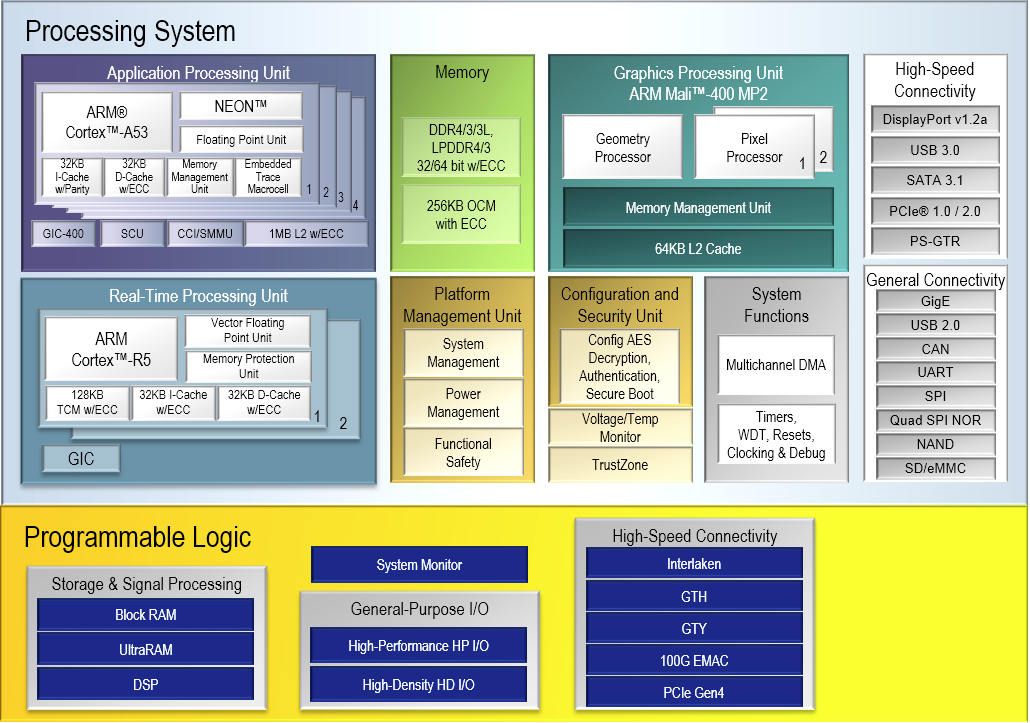
\includegraphics[width=0.75\textwidth]{recursos/mpsoc_arch.png}
    	\caption{Bloques de MPSoC EG}
    	\label{fig:mpsoc_arch}
    \end{figure*}

  \item 2 GB \acrshort{DDR}4 \acrshort{SDRAM}
  \item 64 MB memoria flash \acrshort{QSPI}
  \item 8 GB memoria flash \acrshort{eMMC}
  \item 1 Gigabit Ethernet
  \item 1 conector para tarjetas microSD
  \item 12 conectores \acrshort{PMOD} conectados a la parte de \acrshort{PL}
  \item 1 \acrshort{DIP} switch de 8 posiciones conectado a \acrshort{PL}
  \item 8 LEDs conectados a \acrshort{PL}
  \item 1 conector \acrshort{JTAG}
  \item 2 \acrshort{USB}-\acrshort{UART}
\end{itemize}

\begin{figure*}[h]
	\centering
	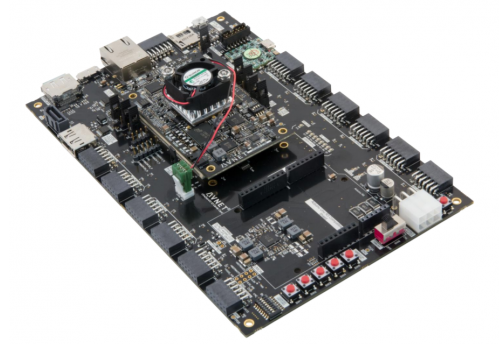
\includegraphics[width=0.65\textwidth]{recursos/ultrazed-eg-carrier.png}
	\caption{UltraZed\texttrademark IO Carrier Card}
	\label{fig:ultrazed-eg-carrier}
\end{figure*}

\subsection{Configuración de SoC} \label{vivado_config}

En la plataforma electrónica que se ha especificado, el componente principal y sobre el que se van a ejecutar los programas y pruebas que se desarrollen es el UltraScale+\texttrademark MPSoC. Este componente dispone de una parte de \acrshort{PS} en la que se encuentran los 4 núcleos ARM Cortex-A53 en los que se van a ejecutar las celdas o dominios en los que se va a dividir el sistema virtualizado. Respecto a la zona de \acrshort{PL}, se va a utilizar como mero instrumento de medida y entrada/salida. En la figura \ref{fig:vivado_1} aparece el diseño de bloques que se ha implementado:

\begin{figure*}[h!]
	\centering
	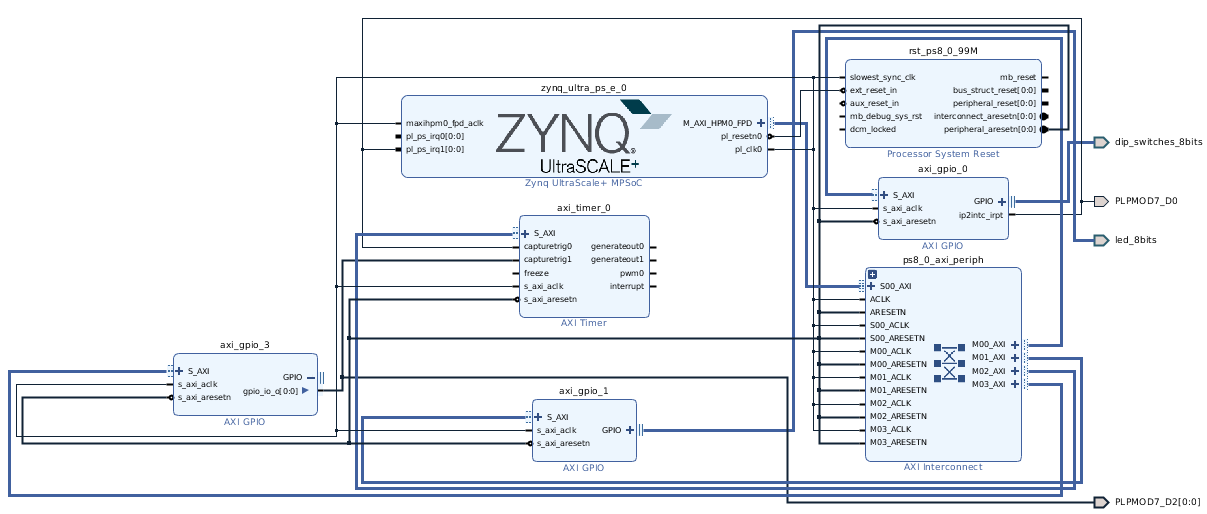
\includegraphics[angle=90,width=\textwidth,height=\textheight,keepaspectratio]{recursos/vivado_1.png}
	\caption{Diseño de bloques de Vivado}
	\label{fig:vivado_1}
\end{figure*}

Como se puede observar, se trata de un sistema muy sencillo en el que todos los bloques se conectan por bus AXI y por tanto aparecen mapeados en memoria del microprocesador. El objetivo es medir la latencia que introducen los hipervisores en el tratamiento de interrupciones en sistemas guest baremetal y con ese fin se han dispuesto los siguientes bloques y conexiones entre ellos.\\

Se ha tomado como generador de interrupciones el cambio en el valor del la entradas del bloque \acrshort{AXI} \acrshort{GPIO} con nombre \textit{axi\_gpio\_0}.
En este bloque se ha habilitado la salida de la interrupción y se ha conectado al grupo de interrupciones de \acrshort{PL} a \acrshort{PS} número 1 (línea verde en la figura \ref{fig:vivado_1}). Este grupo de interrupciones tiene unos números de interrupción que luego tendrán que ser gestionados desde el programa. Estos números los determina la propia arquitectura de Xilinx y ARM. En el presente caso la interrupción es la número 136 \cite{axi_trm}. Más adelante se verá como se utiliza este número en el software.\\
La entrada del bloque \textit{axi\_gpio\_0} está conectada a la salida de un temporizador con nombre \textit{axi\_timer\_1} que se va a configurar en modo \acrshort{PWM} a fin de generar interrupciones periódicas (línea morada en la figura \ref{fig:vivado_1}).


Con objeto de medir con precisión la latencia introducida se ha utilizado un bloque \acrshort{AXI} Timer \cite{axi_timer}. Este bloque se configura en modo captura y como se puede ver en el diagrama, una de las entradas de captura es la interrupción generada por el bloque \acrshort{AXI} \acrshort{GPIO} descrito anteriormente. La otra señal de captura la genera el bloque \textit{axi\_gpio\_3}. La idea principal detrás de esta configuración es poder capturar el valor del contador del Timer en el momento en el que se produce la interrupción y también en el momento en el que la rutina de atención a la interrupción entra y activa la salida de \textit{axi\_gpio\_3}. La diferencia entre estos dos valores es el tiempo que se tarda en atender a la interrupción.

El bloque \acrshort{AXI} \acrshort{GPIO} con nombre \textit{axi\_gpio\_1} tiene su salida conectada a los diodos LED conectados a PL disponibles en la UltraZed. Estos LEDs se han utilizado simplemente como instrumento de verificación visual de que se están ejecutando los programas como se espera.\\

También se ha utilizado uno de los conectores \acrshort{PMOD} para poder monitorizar las señales en curso con un analizador lógico a fin de poder comprobar que los resultados obtenidos de la resta de tiempos en el Timer son coherentes.\\

En la configuración de la zona de PS se han utilizado las definiciones de tarjeta que están alojadas en \url{https://github.com/Avnet/bdf}. Estas definiciones configuran el MPSoc para el \acrshort{SOM} de UltraZed\texttrademark que se está empleando.

\subsection{Otros}

\begin{itemize}
  \item Analizador lógico de 8 canales: con el objeto de realizar algunas medidas empíricas de tiempos de reacción de los hipervisores se ha utilizado como ayuda el siguiente analizador:\\
  \url{https://eur.saleae.com/products/saleae-logic-8}
  \\Algunas de las medidas se han realizado con temporizadores como se verá posteriormente. Aún así el analizador ha servido de apoyo a la hora de comprobar que los resultados obtenidos de los temporizadores eran correctos.
  \item Cable JTAG-HS2: a fin de cargar de forma dinámica y depurar los programas que se han hecho se ha empleado el siguiente debugger apto para productos de Xilinx.\\

  \url{https://www.digikey.es/es/product-highlight/d/digilent/jtag-hs2-programming-cable}
\end{itemize}

\section{Herramientas Software}

A continuación se listan las herramientas software que se han empleado en la elaboración de los tests en los hipervisores Xen y Jailhouse. Para la plataforma electrónica seleccionada ha sido suficiente la licencia gratuita (WebPACK) que proporciona Xilinx.

\begin{itemize}
  \item Vivado Design Suite 2018.3: este paquete de software de Xilinx es el que permite generar lo que se denomina la \textit{Hardware Platform} y exportarla a fin de poder crear proyectos de software sobre ella como se verá más adelante. Esta \textit{Hardware Platform} contiene tanto la parte de configuración de la parte de PS del Zynq\textregistered UltraScale+\texttrademark MPSoC como el bitstream que se programa en la zona PL.\\
  \url{https://www.xilinx.com/products/design-tools/vivado.html}
  \item Xilinx Software Development Kit (XSDK) 2018.3: la herramienta \acrshort{XSDK} es un entorno integrado de desarrollo basado en eclipse que permite desarrollar aplicaciones para ejecutarse sobre la plataforma generada por Vivado. Mediante un sencillo interfaz gráfico se pueden crear aplicaciones tanto baremetal, como FreeRTOS y Linux. Soporta todas las familias de microprocesadores existentes en las plataformas de Xilinx: MicroBlaze, ARM Cortex-R5, ARM Cortex-A9 y ARM Cortex-A53. Cabe destacar que también incorpora un sistema de depurado de software y herramientas de análisis de rendimiento.\\
  \url{https://www.xilinx.com/products/design-tools/embedded-software/sdk.html}
  \item Petalinux Tools 2018.3: en este paquete se proporcionan todas las herramientas y componentes software para construir un sistema embebido basado en Linux en las plataformas de Xilinx.\\
  Desde las últimas versiones su sistema de compilación y generación de software está basado en el proyecto yocto (\url{https://www.yoctoproject.org/}). Xilinx añade una capa software sobre yocto para manejar las particularidades de sus productos.\\
  \url{https://www.xilinx.com/products/design-tools/embedded-software/petalinux-sdk.html}
\end{itemize}

Todas estas herramientas software así como los procesos de configuración, compilación, interacciones con la tarjeta electrónica, etc. se han realizado en una máquina host Linux con sistema operativo Ubuntu 16.04 LTS.
